\documentclass[11pt]{beamer}
\usetheme{Warsaw}
\usepackage[utf8]{inputenc}
\usepackage[brazil]{babel}  % idioma
\usepackage{amsmath,amsfonts,amssymb,textcomp}
\usepackage{graphicx}
\usepackage{subfigure}

\author{Othon Oliveira}
\title{Sistemas Operacionais}
%\setbeamercovered{transparent} 
%\setbeamertemplate{navigation symbols}{} 
%\logo{} 
\institute{Fatec -- Faculdade de Informática --- PE} 
%\date{} 
%\subject{} 
\begin{document}


% Capa - requer o TikZ
\newcommand{\capa}{
    \begin{tikzpicture}[remember picture,overlay]
        \node at (current page.south west)
            {\begin{tikzpicture}[remember picture, overlay]
                \fill[shading=radial,top color=orange,bottom color=orange,middle color=yellow] (0,0) rectangle (\paperwidth,\paperheight);
            \end{tikzpicture}
          };
    \end{tikzpicture}
}


\begin{frame}
\titlepage
\end{frame}

%\begin{frame}
%\tableofcontents
%\end{frame}



%+++++++++++++++++++++++++++++++++++++++++++++++
\begin{frame}{Exemplos de sistemas operacionais}
\begin{figure}[h]
%\left

\includegraphics[width=18mm, height=15mm]{Figuras/appleOficial.jpg}
\qquad \quad \quad \quad \quad

\includegraphics[width=19mm, height=17mm]{Figuras/windows.png}
\qquad \quad \quad \quad \quad \quad \quad 	\vspace{1.0in}

\includegraphics[width=15mm, height=15mm]{Figuras/android.jpg}
\qquad \quad \quad \quad \quad \quad \quad \quad 

\includegraphics[width=25mm, height=15mm]{Figuras/ubuntu_904.jpg}

\end{figure}
\end{frame}

%+++++++++++++++++++++++++++++++++++++++++++++++
\begin{frame}{Conceito}
	\begin{itemize}
	\item[1-] Programas ?
	\vspace{0.2in}
	\item[2-] Processos ??
	\end{itemize}
\end{frame}


%+++++++++++++++++++++++++++++++++++++++++++++++
\begin{frame}{Programas}
	MS-Word, Google-Chrome, Firefox, Whatsapp,...
\begin{figure}[h]
%\left

\includegraphics[width=18mm, height=15mm]{Figuras/Firefox-logo.png}
\qquad \quad \quad \quad \quad \quad \quad

\includegraphics[width=19mm, height=17mm]{Figuras/IE.png}
\qquad \quad \quad \quad \quad \quad \quad

\includegraphics[width=45mm, height=15mm]{Figuras/whatsapp10.png}
\end{figure}
\end{frame}


%+++++++++++++++++++++++++++++++++++++++++++++++
\begin{frame}{System Calls}
\begin{itemize}
 \item Programas solicitam serviços ao sistema opercional através de \textbf{Chamadas de Sistemas} 
 \item Programas bem escritos informam ao sistema oparacional exatamente do que necessitam
 \item Na compilação são passadas informações geralmente ``escondidas'' nas bibliotecas do sistema, exemplo: printf() -- linguagem C
\end{itemize}
\end{frame}


%+++++++++++++++++++++++++++++++++++++++++++++++
\begin{frame}{Principais componentes do Kernel}
A parte do sistema operacional responsável pelas chamadas de sistema é o núcleo ou \textit{Kernel}
\begin{itemize}
 \item gerência de processos *
 \item gerência de memória
 \item sistema de gerência de arquivos \textit{filesystem}
 \item gereência de entrada e saída
\end{itemize}
\end{frame}


%+++++++++++++++++++++++++++++++++++++++++++++++

\begin{frame}{Programas X Processos}
Programas: conjunto de instruções que descrevem tarefas para serem executadas num computador\\
\vspace{0.4in}
Processos: um programa sendo executado + dados necessários a sua execução

É de responsabilidade do sistema operacional gerir os processos do sistema de forma a maximizar a 
utilização da CPU.
\end{frame}



%+++++++++++++++++++++++++++++++++++++++++++++++
\begin{frame}{Processos}
\begin{figure}[h]

\subfigure{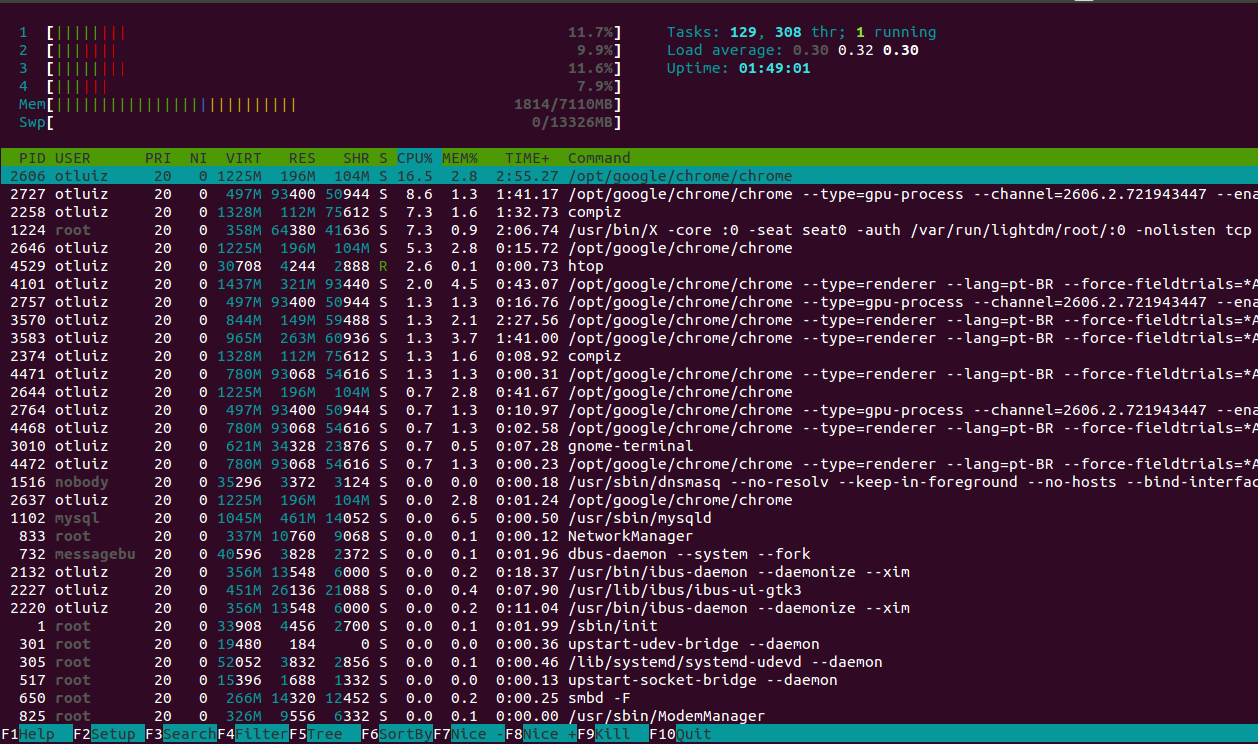
\includegraphics[width=61mm, height=40mm]{Figuras/processos.png}}
%\qquad \quad \quad \quad \quad \quad \quad
\subfigure{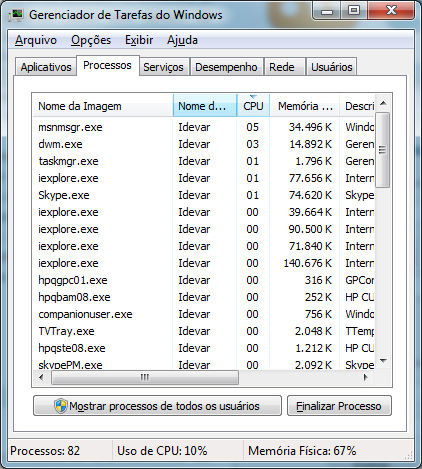
\includegraphics[width=36mm, height=42mm]{Figuras/gerenciadortarefas.png}}
\end{figure}

%Processos: Um programa sendo executado
\end{frame}



%+++++++++++++++++++++++++++++++++++++++++++++++
\begin{frame}{Atributos}
Um processo contém um contexto que o identifica:
 \begin{itemize}
 \item PID : um número inteiro que o indentifica
 \item UID : o usuário que o criou 
 \item CPU : percentual da CPU que está utilizando
 \item MEM : percentual da memória que está sendo usado
 \item STS : o estado do processo naquele momento
 \item PRI : a prioridade que o processo tem para ser executado
 \item TMP : o horário que foi chamado
 \item CMD : o comando que o chamou
 \item xxx : ...

 \end{itemize}
\end{frame}



%+++++++++++++++++++++++++++++++++++++++++++++++
\begin{frame}{Estados de um processo}
\begin{itemize}
 \item Criado (ou iniciado)
 \item Apto (ou ready para ser executado)
 \item Executando (ou running)
 \item Esperando	  (ou waiting)
 \item Bloqueado (ou stopped)
 \item Destruído (ou dead)
 \item Zumbi (ou zombie)
\end{itemize}
\end{frame}

%+++++++++++++++++++++++++++++++++++++++++++++++
\begin{frame}{Estados dos processos}
\begin{figure}[h]
 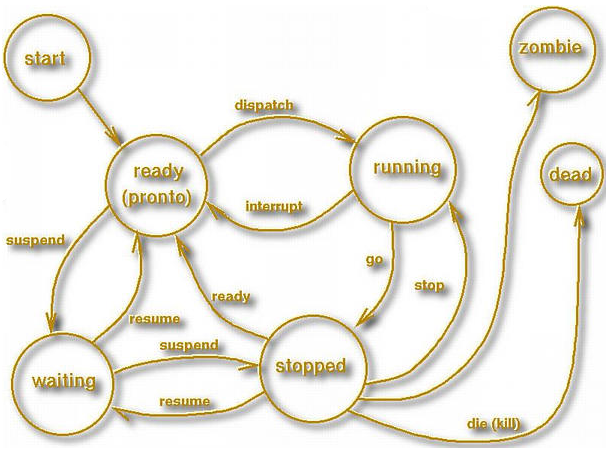
\includegraphics[width=61mm, height=40mm]{Figuras/statusProc.png}
\end{figure}
O sistema operacional ``pega'' um processo na fila de aptos para receber o processador.
O processo passa do estado ``apto'' para ``executando''.
O módulo do sistema operacional que faz essa seleção é o \textbf{Escalonador} (\textit{Scheduler})
\end{frame}

%+++++++++++++++++++++++++++++++++++++++++++++++
\begin{frame}{Tipos de processos}
 Processos são criados e destruídos a todo tempo. O momento e a forma como eles são criados depende do sistema operacional considerado.
 A forma mais comum é permitir que os processos sejam criados livremente, através das chamadas de sistemas.
 A maioria de processos de um sistema operacional executam programas de usuários, entretanto alguns processos podem realizar tarefas do sistema.
\end{frame}

%+++++++++++++++++++++++++++++++++++++++++++++++
\begin{frame}{Deamons}
 Os processos do sistema (deamons) controlam autonomamente os recursos da máquina, são iniciados quando o computador ou quando chamamos, por exemplo, uma técnica chamda spooling copia os arquivos a serem impressos para a impressora, fazendo com que os arquivos na fila de impressão não precisam esperar pela impressora, dando a sensação de que o programa de usuário foi quem executou isso. Esse processo não está associado a nenhum programa de usuário, é próprio do sistema operacional.
\end{frame}

%+++++++++++++++++++++++++++++++++++++++++++++++
\begin{frame}{Processos Interativos}
 São processos iniciados a partir de um sessão de terminal de comandos e por ele será terminado.
 Quando iniciamos um processo pelo terminal estamos rodando um processo em foreground.
 Um processo em foreground recebe diretamente do terminal(ou stdin) comandos que o controla.
 A saída(stdout ou stderr) também vêm via terminal.
 Um processo em backgound não estão apto a receber instruções diretamente, ele executa normalmente sem interrupções do usuário.
\end{frame}

%+++++++++++++++++++++++++++++++++++++++++++++++
\begin{frame}{Processos em lote -- \textit{batch}}
 Processos em \textit{batch} são controlados usualmente por um programa (cron no Linux). O programa Cron executa uma série de comandos pré-definidos usuário, exemplo: como o programa > at 18:30 xxx, será executado o programa xxx às 18h30. Uma séria de comandos podem estar encadeados para serem executados em lote.
\end{frame}


%+++++++++++++++++++++++++++++++++++++++++++++++
\begin{frame}{Simulação de um processo}
 Terminal de comandos do Linux com o comando \textbf{top} (ou htop) 
 Terminal de comandos do Linux com o comando \textbf{ps -aux}
\end{frame}

%+++++++++++++++++++++++++++++++++++++++++++++++
\begin{frame}{Vídeo}
 Apagar as luzes, por favor !!!
\end{frame}



\end{document}